\chapter{Data Preprocessing}

\section{Feature Selection}

Data collection is simply a process of fetching the data from the data source. However, feature selection is a process of selecting fields from which the target field will be predicted. Suppliers provide stock details along with associated product taxonomy. Importing well-defined taxonomy requires to train the classification model with already existing correct pair of features and label. The already existing pair of features and the correct label for each input is the training data set or training corpora. The classifier built on such a training corpora is termed as supervised classification \parencite{BirdKleinLoper09}.

\begin{figure}[H]
      \centering    
      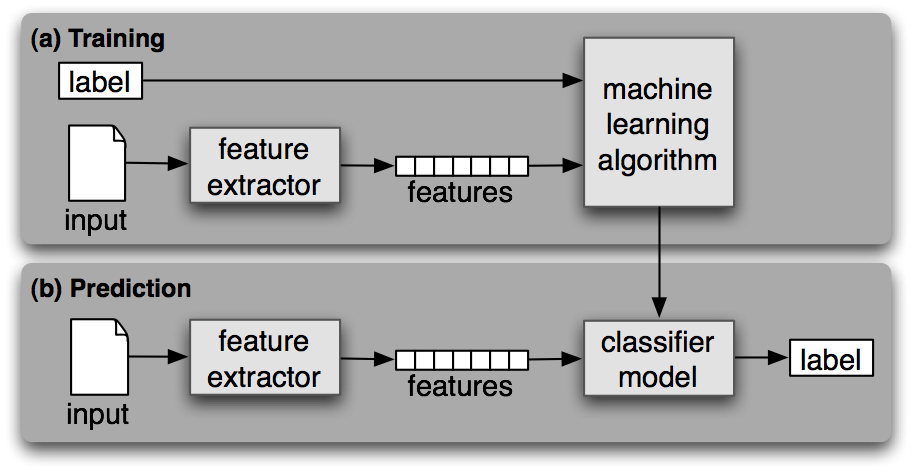
\includegraphics[scale=0.9]{supervised-classification.png}
      \caption{Supervised classification \parencite{BirdKleinLoper09}}
      \label{fig:supervised-classification}
  \end{figure}

  As illustrated in figure \ref{fig:supervised-classification}, during training, a pair of feature set and label are fed in to the machine learning algorithm to generate a classifier model. During prediction, same feature set are fed into the model to predict the label. Refer to chapter \ref{ch:feature-extraction} for details on feature extraction.

In this project, author choose to create a classification model with only one feature that is the name of the product. However, author identifies the potential features to classify the target of n levels of category. These features have been identified based on the understanding of domain of the product. For products with many details will have many more features to be taken into consideration. In such case, selection based on common understanding of the nature of the product may not be sufficient. Hence, Scikit learn  \parencite{sklearn_api} provides methods to define feature appropriately. 


\subsection {Feature Selection Methods} \label{sec:feature-selection}

A feature represents a dataset fine-tuned to serve as a training data for machine learning model. Choosing obvious set of features could get a decent performance on classification task. However, carefully constructed relevant set of features could impact the learning ability and have a significant gain in performance. The feature selection API from Scikit learn \parencite{sklearn_api} also refers to it as dimensionality reduction. 

\parencite{BirdKleinLoper09}  describes some approaches for feature selection as following:

\begin{itemize}
      \item Kitchen sink 
      

      All the features are initially included later each are checked to determine whether they are actually helpful.

      \item Error analysis
      
      The data corpus is split into development-set and test-set. Development-set is subdivided into training set and dev-test set. Training set is used to train the model, dev-test set is employed for error analysis.  The individual error cases are examined for wrongly predicted labels.
      
      
      \begin{figure}[H]
            \centering    
            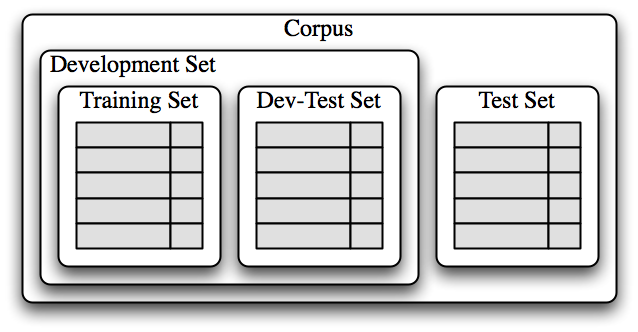
\includegraphics[scale=0.5]{corpus-org.png}
            \caption{Corpus organization for supervised classification \parencite{BirdKleinLoper09}}
            \label{fig:corpus-supervised-classification}
        \end{figure}

\end{itemize}

 Methods for feature selection with Scikit Learn API are:-
\begin{itemize}
      \item Removing features with low variance
      \item Univariate feature selection
      \item Recursive feature elimination

\end{itemize}
\clearpage
\subsection{Obvious Feature Selection}

In this paper, the datasets used are of an ecommerce business specializing in automotive industry domain. Secondary dataset used is from the TecDoc catalogue by TecAlliance \footnote{https://www.tecalliance.net/}. 

Table \ref{table:feature_decription} lists the obvious features for an ecommerce domain. In this paper, five levels of categories are taken into consideration. The number of category levels differ for each product. Consider an example of category tree with three levels. 

\begin{quote} 
\centering 
sparepart/cooling-system/thermostat
\end{quote}
In this example, the lowest level of category is ``thermostat'' as level 4 and level 5 does not exist and will be represented by black or NaN. These blank or NaN value records can go through data imputation as discussed in chapter \ref{ch:data-imputation}.



\begin{table}[h]
      \centering
      \caption{Feature description}
      \label{table:feature_decription}
      \begin{tabular}{ lll }
            \toprule
            
            \textbf{No}& \textbf{Feature} & \textbf{Description}\\
            \midrule
            1&Product name & normalized form of name\\
            2&Category tree & multi level categories\\
            3&Description & Description with html tags\\         
            4&Short description  & product info displayed\\
            5&Supplier  &  supplier of the product\\
            6&Manufacturer  &  manufacturer of the product\\           
            7&Price  &  Price of the product\\
            8&Dimension  & Height, weight of the product\\
            9&(n-1) number of  category levels   &  n is the total category level, one of which will be the target\\
           
            \bottomrule
            \end{tabular}


\end{table}

\subsection {Fetch Existing Product Taxonomy (Corpus) using Elasticsearch}
Elastic search \footnote{https://www.elastic.co/} is a fast and scalable search and analytics engine. It can build a powerful AI and machine learning enabled search experience. In this paper, author fetches labeled dataset of products to serve as the training data for the machine learning.


The above code fetches indexed product name and its lowest hierarchy level category.  
\begin{table}[h]
      \caption{Index: english-name-category statistics}
      \centering
      \label{table:enc}
\begin{tabular}{ll}
      \toprule 

      Samples total&22160 \\
      Dimensionality&2 \\
      Features&name \\
      Label&category \\
      
      \bottomrule
\end{tabular}
\end{table}

Table \ref{table:enc} highlights the total number of products and category and name of fields considered as feature and label. 

\clearpage
\section{Text Normalization} \label{text_normalization}

Text normalization is a process of transforming the document into a standard and consistent form of a text. A document is a text from single source. Some examples of document are list of product names from databases, a pdf file, texts retrieved from web scraping. Text normalization enables to perform required operations on the text as the text inputs are consistent across the document. The process of text normalization varies based on the type of text that needs to be normalized. There is no standard method for text normalization task. In this paper, text normalization of product name and category from the database source is performed. 

In table \ref{table:TN}, displays the difference in text before and after normalization. 

\begin{table}[h]
      \caption{Sample of text normalization effect}
      \centering
      \label{table:TN}
\begin{tabular}{lll}
      \toprule 
                  &\textbf{Name} & \textbf{Category} \\ 
      \midrule
      \textbf{Before}& Company V10-4245 Stoßdämpfer & Stoßdämpfer \\
      \textbf{After}&company v104245 stossdaempfer & stossdaempfer \\
      
      \bottomrule
\end{tabular}
\end{table}

\subsection{Lower Case Conversion}

Using Pandas - vectorized string method, a text can be lower cased across the document. These methos exclude the missing  / NA values automatically \parencite{mckinney-proc-scipy-2010}, shown in code \ref{code:pvsm}.

\begin{lstlisting}[language=Python, caption={Pandas vectorized string method },label={code:pvsm}]
      df_de["name"]= df_de["name"].str.lower()
\end{lstlisting}

\subsection{HTML Parsing}

Probability of getting HTML tags in a document increases if the source of document is from web scraping or also if the document from database source has inline HTML tags. In such case, fetching normal texts from an HTML text is required. One of the method would be to use regular expressions to get text in between angel brackets \textless \textgreater text \textless \textgreater, as in code \ref{cd:html}. However, this method would require to have the tags to be well-formed.
\begin{lstlisting}[language=Python, caption={Regular expression to get text from html},label={cd:html}]
      text = re.sub('<[^>]*>', '', text)
\end{lstlisting}



The better option would be to use Beautiful Soup \footnote{https://www.crummy.com/software/BeautifulSoup/bs4/doc/} a Python library for pulling data out of HTLM and XML, using code \ref{cd:bs}.
\begin{lstlisting}[language=Python, caption={Beautiful soap API to get text from html},label={cd:bs}]
      # Remove html tags 
      soup = BeautifulSoup(doc, 'html.parser')
      text =soup.get_text()
\end{lstlisting}
\clearpage
\subsection{Cleaning Text}
A product detail text may contain non-word characters represented in regular expression as \textbackslash W. It may also contain space separated decimals describing the dimensional values of the product such as weight, height. Regular expressions could be used for removing the non-character words and spaces between the decimal values, using code \ref{cd:ct}. 

\begin{lstlisting}[language=Python,,caption={Clean text with Regular expression},label={cd:ct}]
      text = (re.sub('[-\W]+', ' ', text))
      text = (re.sub('(?<=\d) (?=\d)', '', text))
\end{lstlisting}

\subsection{Normal form D - Unicode database}

A product name in Deutsch language may contain umlaute characters such as \"A.  Pythons unicodedata \footnote{https://docs.python.org/3/library/unicodedata.html} module provides access to the Unicode Character Database (UCD) which defines the character properties for all Unicode characters. To change \"A to A, the Normal form D (NFD) should be applied which translated each character into its decomposed form. Further the text can be refined with the general category assigned to the character as string. Nonspacing mark characters \footnote{https://www.compart.com/en/unicode/category/Mn} are represented as ``Mn''. These characters could be removed by referring the character category as shown in code \ref{cd:nd}.
\begin{lstlisting}[language=Python ,caption={NFD normalization},label={cd:nd}]
      ''.join(
            c for c in unicodedata.normalize('NFD', text)
            if unicodedata.category(c) != 'Mn')
\end{lstlisting}

Another option is to replace the German characters to equivalent English sounding characters. Table \ref{table:deu-eng} lists the common German characters and their equivalent English sounding series of characters. In this way, the reverse translation is easier.
\begin{table}[h]
      \centering
      \caption{German characters to English}
      \label{table:deu-eng}
      \begin{tabular}{ llll }
            \toprule
            \"A& Ö&  Ü&ß \\
            Ae&Oe & Ue&ss\\         
          
            \bottomrule
            \end{tabular}
  \end{table}


  \subsection{Avoided normalization processes}

  In this project, some commonly practiced normalization process are being avoided. Which once and why are described below.

  \begin{itemize}
      \item Stemming 
      
      Stemming is a process of striping off any affixes. \acl{nlp} tools such as NLTK provide stemmers. The Porter and Lancaster
      stemmers follow their own rules for stripping affixes \parencite{BirdKleinLoper09}. Author required not to deviate from the original vocabulary of features.

      \item Lemmatization
      
      Lemmatization remove the affixes if the word is in the used libraries' dictionary. The vocabulary for corpora and any third party library such as WordNet cannot be synced.   

  \end{itemize}



\section{Impute missing text data} \label{ch:data-imputation}

Machine leaning algorithms requires that their inputs have no missing values.
Missing values encoded as NaNs or blanks are incompatible with estimators which represents as the numerical values and assumes all values have and hold meaning. Discarding the entire row and/or columns of a dataset containing the missing values could lead to losing valuable data. The process to fill (impute) missing values are referred to as imputation.

\subsection{Feature imputation / Regression imputation or \\ Predictive Imputation}

Machine learning algorithm to predict values in a categorical variable based on other available features. Table \ref{table:feature_imputation} states the categorical features from the all the features mentioned in \ref{table:feature_decription}.


\begin{table}[h]
    \centering
    \caption{Identify categorical features}
    \label{table:feature_imputation}
    \begin{tabular}{ lll }
          \toprule
          
          \textbf{No}& \textbf{Feature} & \textbf{Categorical}\\
          \midrule
          1&Product name & No\\
          3&Description & No\\         
          4&Short description  & No\\
          5&Supplier  & Yes\\
          6&Manufacturer  &  Yes\\           
          7&Price  &  No \\
          8&Dimension  & Yes\\
          \bottomrule
          \end{tabular}
\end{table}

The \textit{dimension} column is also considered as a categorical value as it has few unique values.

If \textit{supplier} is the missing value from the set of row. The missing \textit{supplier} data must be predicted only from the available list of suppliers. A supervised machine learning with labeled dataset to train the model to classify the available features data to predict \textit{supplier}. A tensor size of the number of unique \textit{supplier} will be the output of the model. 
In an iterated round-robin fashion, at every step a missing feature column  \textit{y} and other feature columns treated as input \textit{x} predicts the missing values of \textit{y}. Regression imputation is more accurate than mode imputation on categorical value.


\subsection{Mode imputation}

Replacing the most frequent categorical value in a column is known as mode imputation.  Pandas.DataFrame.mode \parencite{mckinney-proc-scipy-2010} function returns most often value. Code snippet \ref{cd:ml} will fill the missing values for each column using its own most frequent value.

\begin{lstlisting}[language=Python, caption={Pandas DataFrames mode function},label={cd:ml}]
    df = df.fillna(df.mode().iloc[0])
\end{lstlisting}

Mode imputation on categorical data are prone to fill incorrect data if the missing data is not the most frequent one.


\clearpage
\subsection{\acf{KNN}  imputation}

\acl{KNN} is a supervised learning algorithm and is used to search dataset with the most similar elements to a given query element, with similarity defined by a distance function. This imputation method is suitable for categorical data.

The most common distance metrics functions are:-

\begin{enumerate}
    \item Euclidean distance.
    % \begin{lstlisting}[language=Python, caption={Euclidean distance formula }]
    %     dist(x, y) = sqrt(dot(x, x) - 2 * dot(x, y) + dot(y, y))
    %         \end{lstlisting}
    \item Manhattan distance.
    \item Hamming distance.
\end{enumerate}

sklearn.neighbors.KNeighborsClassifier \parencite{scikit-learn} does an instance-based learning, it does not construct a model, but stores instance of training data. Classification is computed from majority vote of nearest neighbors of each point.

The \textit{k}-neighbors classification implements learning based on  \textit{k} nearest neighbors of each query point, where \textit{k} is integer value specified by user. The optimal \textit{k} value can be evaluated by iterating the classifier with different  \textit{n\textunderscore neighbors} Parameter and finding the minimum value of error rate, refer code \ref{cd:kn}. Larger \textit{k} suppresses the effects of noise, but makes the classification boundaries less distinct.

\begin{lstlisting}[language=Python, caption={Find optimal \textit{k} value in \acl{KNN} },label={cd:kn}]
    error_rate = []
    for i in range(1,40):
        knn = KNeighborsClassifier(n_neighbors=i)
        knn.fit(X_train,y_train)
        pred_i = knn.predict(X_test)
        error_rate.append(np.mean(pred_i != y_test))

    print("Minimum error:-",min(error_rate),"at K =",error_rate.index(min(error_rate)))
\end{lstlisting}



\subsection{\acs{KNN} model implementation}

In table \ref{table:KNN_implementation} there are 7 columns. Target column is \textbf{Category-Level-3} which is the category at level three.
As per the example category hierarchy in table \ref{table:KNN_implementation} 



\begin{table}[h]
    \centering
    \caption{Sample features }
    \label{table:KNN_implementation}
    \begin{tabular}{ll}
        \toprule     
        \textbf{Name}& \textit{product name} \\
        \textbf{Description}& \textit{product description} \\
        \textbf{Short-Description}& \textit{product short description} \\
        \textbf{Category-Level-1}& Spare-Part \\
        \textbf{Category-Level-2}& Cooling System \\
        \textbf{Category-Level-3}& Thermostat \\
        \textbf{Category-Level-4}& NaN \textit{product has no level 4 category} \\
        \bottomrule
    \end{tabular}

\end{table}

\begin{lstlisting}[language=Python,caption={Finding k-nearest neighbor},label={cd:fkn}]
    from sklearn import preprocessing
   
    X = df.drop(['catL3'], axis = 1)
    y = df['catL3']

    X = preprocessing.StandardScaler().fit(X).transform(X.astype(float))
    from sklearn.model_selection import train_test_split
    X_train, X_test, y_train, y_test = train_test_split( X, y, test_size=0.2, random_state=4)
    from sklearn.neighbors import KNeighborsClassifier
    from sklearn import metrics
    #Train Model and Predict
    k = 3  
    neigh = KNeighborsClassifier(n_neighbors = k).fit(X_train,y_train)
    Pred_y = neigh.predict(X_test)
    print("Accuracy of model at K=3 is",metrics.accuracy_score(y_test, Pred_y))
\end{lstlisting}


Code snippet \ref{cd:fkn} performs the following tasks:

\begin{itemize}
    \item Collect independent data features into the X data frame and target field into a y data frame.
    \item  Split data into training and testing. 
    \item  Import the classifier model from sklearn library and fit the model with  \textit{k} value equal to the optimal value.
\end{itemize}




\subsection{Mean/median imputation}

Pandas.DataFrame.median \parencite{mckinney-proc-scipy-2010} returns the median value, refer code \ref{cd:mim}. These can be applied to the features represented in numerical value. In reference to table \ref{table:feature_imputation}, \textit{price} could be a column on which median value can be filled. However, using median to fill missing value could underestimate or overestimate the value.

\begin{enumerate}
    \item Median - The mid point value
    \item Mean - The average value
\end{enumerate}

\begin{lstlisting}[language=Python,caption={Mean imputation},label={cd:mim}]
    df = df.fillna(df.median().iloc[0])
\end{lstlisting}

\section{Log transformation of data}

Log transformation is a mathematical operation applied on data to change its scale and to reduce its skewness and to make data more symmetric.  Skewness is a measure of the asymmetry of a distribution, and a right-skewed distribution has a long tail on the right side of the distribution \parencite{BonnieMa}. The Numpy library provides natural logarithmic function to apply log transformation on array of data.


\section{Feature extraction} \label{ch:feature-extraction}

Transforming text or image data into numerical representation usable for machine learning is called feature extraction. Raw sequence of data cannot be fed directly into a machine learning algorithm as they expect data in numerical vector and in fixed size. Whereas raw text document are of variable lengths. 

\subsection{Count Tokenization}

Tokenization is splitting the text in sequential words which can be embedded in a vector space.
For example, the normalized product name ``abc joint kit drive shaft'' can be tokenized into  ``abc'',``joint'',``kit'',``drive'',``shaft''. Number of occurrence of each token in a document is called counting in terms of numerical feature extraction.

\subsection{Count Vectorization or One-Hot encoding} \label{ch_countvector}


CountVectorizer class of scikit learn API implements both tokenization and occurrence counting \parencite{sklearn_api}. 

Consider a data frame with columns \textit{ProductName} and data value as in tbale \ref{table:count_vectorization}

\begin{table}[h]
    \centering
    \caption{Sample data for count vectorization}
    \label{table:count_vectorization}
    \begin{tabular}{ l }
          \toprule
          
          \textbf{ProductName}\\
          \midrule
          abc joint kit drive shaft\\
          xyz joint kit drive shaft\\
         
          \bottomrule
          \end{tabular}
\end{table}

The length of the vocabulary is the number of unique tokens in the data frame column. In the sample data the vocabulary length is six. The vector has the dimensionality equal to the size of the vocabulary. Adding one in the dimension to each of the word in the vocabulary represents one hot encoding.

\begin{table}[]
    \centering
    \caption{Sample One-Hot encoding}
    \label{table:countencode}
    \begin{tabular}{ ll }
          \toprule
          
          \textbf{text}& \textbf{encoding}\\
          \midrule
          abc&[1,0,0,0,0,0]\\
          joint&[0,1,0,0,0,0]\\
          kit&[0,0,1,0,0,0]\\
          drive&[0,0,0,1,0,0]\\
          shaft&[0,0,0,0,1,0]\\
          xyz&[0,0,0,0,0,1]\\
       
          \bottomrule
          \end{tabular}
\end{table}

\subsection{ \textit{n-grams} Vectorization} \label{sec:ngram_vector}

Count Vectorization can also be performed on range of grams of words. 

\begin{lstlisting}[language=Python,label=ngramcode, caption={\textit{n-gram} vectorization},label={cd:cv}]
    bigram_vectorizer = CountVectorizer(ngram_range=(1, 2))
    bigram_vectorizer.fit(df["ProductName"])
\end{lstlisting}


The code in listing \ref{cd:cv}, will add additional vocabularies of two words such as "drive shaft". This enables to preserve local ordering information. 

\subsection{Pickling the Vectorizer} \label{pickle_vector}

Pickle \footnote{https://docs.python.org/3/library/pickle.html} module creates a portable serialized representation of python object. Reusing the CountVectorizer object once it has been fit with the document can be enabled by Pickle module, refer code \ref{cd:pv}. 

\begin{lstlisting}[language=Python,label=pickle, caption={Pickle vectorization},label={cd:pv}]
    pickle.dump(self.vectorizer, open("vector.pickel", "wb"))
\end{lstlisting}

The memory use will grow as the vocabulary in the text corpus grows.  Pickling and un-pickling of vectorizer will slow for large vocabulary.
This issue can be tackled by hashing the features. 

\clearpage
\section{Summary}

In this chapter, search analytic engine named Elastic search is introduced. The author as a prototype of classification model choose to include only two-dimensionality. One is the feature (product name) and other is the label to be predicted (category.)

Table \ref{table:feature_decription} list the features for determining the product taxonomy. These features are listed based on general knowledge and understanding. However, productive method for refining the feature such as error analysis can be utilized for feature selection. Scikit learn API \parencite{sklearn_api} also provides some functions for feature selection.

Before extracting the features (refer chapter \ref{sec:feature-extraction}) it is important to normalize and standardize the data set. If the text normalization step is skipped then while creating the numerical representation of the text the data will be inconsistent. For example, same text with proper case (Car) or lower case (car) will have two representation even though the semantic meaning is the same.  

The methods involved in text normalization are lower casing the text, removing the HTML tags, removing irrelevant numerical data within the text such as product dimensionality, and making the text across the document with one Unicode database.

Missing input values sometimes denoted as blanks or NaN's cannot be considered for transforming into a numerical representation value. Machine learning algorithm feed in input data as a numerical representation of data terms as extracted features. Removing the missing values from the dataset sometime may not be feasible. As this may lead to loss of vital information of the product. 

Predicting the missing values, replacing the missing value with most frequent values, finding most similar value with K - nearest neighbors, replacing the values with median or mean values are some methods to replace the missing values from the dataset.


Feature extraction is a process of transforming the normalized text into numerical representation for machine learning.  Tokenization of text and Counting are terms to split the text in sequence of words and there occurrence. 

In this thesis, author has used the n-grams vectorization method to convert the feature - product name into a vector format. This creates a vocabulary of product name. For example, consider total number of unique words in entire product name column is 100. The name of the product will be a vector shape of 1 \time 100 with each text represented in one-hot encoded format. Refer table \ref{table:countencode} for visual representation.
